\documentclass{article}
\usepackage{algorithm}
\usepackage{algpseudocode}
\usepackage{amsmath}
\usepackage{amssymb}
\usepackage{amsthm}
\usepackage[titletoc]{appendix}
\usepackage{array}
\usepackage[english]{babel}
\usepackage{booktabs}
\usepackage{cancel}
\usepackage{color}
\usepackage{eqparbox}
\usepackage{float}
\usepackage[margin=1in]{geometry}
\usepackage{graphicx}
\usepackage[colorlinks=true]{hyperref}
% *must* be loaded after hyperref
\usepackage[toc, acronym, numberedsection=nameref]{glossaries}
\usepackage[utf8]{inputenc}
\usepackage{lipsum}
\usepackage{mathtools}
\usepackage[cache=false]{minted}
\usepackage{parskip}
\usepackage{pgfplots}
\usepackage{scalerel}
\usepackage{skull}
\usepackage{subcaption}
\usepackage{titling}
\usepackage{textcomp}
\usepackage{tikz}
\usepackage[compact, explicit]{titlesec}
\usepackage{textcomp}
\usepackage[nottoc]{tocbibind}
\usepackage[textsize=small]{todonotes}
\usepackage[normalem]{ulem}

% Document Settings

\definecolor{__minted_background_color}{rgb}{0.95, 0.95, 0.98}
\definecolor{__minted_highlight_color}{rgb}{0.88, 0.88, 1.0}
\setminted{autogobble=true,
    style=tango,
    breaklines,
    bgcolor=__minted_background_color,
    highlightcolor=__minted_highlight_color,
    mathescape, % Escape math mode everywhere.
    texcomments,  % Enable latex code inside of comments. Useful for referencing equations.
}

\usetikzlibrary{arrows, backgrounds, matrix, positioning, shapes}
\pgfplotsset{compat=1.15}
\numberwithin{equation}{section}
% Sets the width of the margin TODO notes
\setlength{\marginparwidth}{0.84in}
\reversemarginpar{}

% hex #184c9a
\definecolor{__glossary_entry_color}{rgb}{0.094, 0.298, 0.604}
\renewcommand{\glstextformat}[1]{\textbf{\textcolor{__glossary_entry_color}{#1}}}

% Add glos: to the beginning of the glossary labels.
\renewcommand*{\glsautoprefix}{glos:}

% All I want is to have comment italicized, but I cant figure out how
% to properly modify the existing \Comment macro.
% \algrenewcomment[1]{\hfill\eqparbox{COMMENT}{\textit{// #1}}}
\algnewcommand{\IComment}[1]{\Comment{\textit{#1}}}
% enable \autoref with algorithms
\newcommand{\algorithmautorefname}{Algorithm}

% TODO: Should this path be relative to the document root or this file?
\graphicspath{{./figures/}}

% Document Definitions

\newcommand{\C}{\mathbb{C}}
\newcommand{\R}{\mathbb{R}}
\newcommand{\Z}{\mathbb{Z}}
\newcommand{\N}{\mathbb{N}}
\renewcommand{\O}{\mathcal{O}}

\theoremstyle{definition}
\newtheorem{defn}{Definition}[section]

\theoremstyle{plain}
\newtheorem{thm}{Theorem}[section]

\renewcommand{\qedsymbol}{$\skull$}

% An inline TODO command. Doesn't play nicely with \todotableofcontents
\newcommand\todoinline[2][]{\todo[inline, caption={TODO}, #1]{
        \begin{minipage}{\textwidth-4pt}#2\end{minipage}}}

% Draw clouds around things. Useful in mathematical proofs.
\newcommand{\cloud}[4][\dots]{
    \raisebox{-0.4\height}{
        \begin{tikzpicture}
            \node [cloud,
                draw,
                cloud puffs=#2,
                cloud ignores aspect,
                minimum height=#3,
                minimum width=#4] {#1};
        \end{tikzpicture}
    }
}

% % make each \section a problem.
% \titleformat{\section}[runin]{\large\bfseries}{}{0pt}{\titlerule[1.5pt]\newline\vspace*{-4pt}
%     Problem\quad\thesection\newline}[\vspace{0.01ex}{\titlerule[1.5pt]}]

% Make autorefs to sections say "Problem x"
% \AtBeginDocument{%
% \renewcommand{\sectionautorefname}{Problem}
% }

% Use \ceil*{} or \floor*{}
\DeclarePairedDelimiter{\ceil}{\lceil}{\rceil}
\DeclarePairedDelimiter{\floor}{\lfloor}{\rfloor}


\title{Homework 2}
\author{Austin Gill \\ Riley Kopp}

\begin{document}
\maketitle
\begingroup
\hypersetup{linkcolor=black}
\tableofcontents
\endgroup
\newpage

\section{Introduction}\label{sec:introduction}
The problem we were attempting to solve was to generate an approximation to a given image using
$N$ geometric objects. We chose to focus exclusively on approximating grayscale images with
collections of circles.

The intent of this homework was to use novel evolutionary methods to build the image
approximation. Thus we attempted multiple solution strategies from topic discussed in class to
build our approximations. A summary of our notable attempts is given below.

Our first attempt was to use Simulated Annealing to produce a single approximation over time.
Unfortunately, this did not yield immediately gratifying results on even the simplest of images
with about a full day of tuning.

Our second attempt was to implement a vanilla evolutionary algorithm with mutation only (no
recombination). This yielded better results on simple images, but only a small fraction of the
time. One more complicated images, this method failed to yield even slightly reasonable results.
Our guess is that a better mutation method and implementing recombination would improve this
method, but due to tendencies observed in other methods we decided against attempting to improve
this strategy in favor of another.

Our third notable attempt occurred after several hours of discussion with another classmate.
Their attempt yielded incredible results, but was quite complicated. However, the base strategy was
to evolve the image one circle at a time. That is the first circle was evolved over time with
mutation and crossover, then added to the image. Then the second was evolved over time and added to
the image. The end result of this approach is a single approximation of the image, built slowly
over time. Traditional evolutionary methods would have a population of approximations, and would
yield several approximations of the image.

Thus our attempt was to use a greatly simplified version of this approach in parallel to
initialize a population of approximations, each already fairly good, and then to mutate and
reproduce that population. Unfortunately, we observed this approach to do no better than simple
using the initial population. This might be for several reasons, including the small population
size limited by the computational efforts of generating large populations, and the lack of
diversity in the initial population.

In view of these summarized results, we found that our fourth attempt --- implementing a
simplified and greedy circle-by-circle approach --- worked the best.

Lastly, we experimented with layering individuals on top of each other to form composite
images. This was quite effective, especially since the individuals have no dependency between them
and can be trivially parallelized.

\section{Solution Strategies}\label{sec:strategies}

Throughout our implementations, we made use of a Numpy capability not commonly known. It is
possible to create custom datatypes for an array.

\begin{minted}{python}
    # Creates a custom point datatype
    point = np.dtype([('x', 'float32'), ('y', 'float32'), ('color', 'uint8'))])
    # Creates an array of 100 points, zero-initialized
    points = np.zeros(100, dtype=point)
    # Access the parallel array of x's
    xs = points['x']
    # Access the x component of a single point
    points[0]['x']
\end{minted}

According to StackOverflow, the intent of the custom datatypes is to make bookkeeping of parallel
arrays easier, not to treat the array as a single array of structs. Using the custom datatypes made
some operations much easier, but overall caused much more trouble than what they were worth.

For example, the popular Numba library, which provides a just-in-time compiler for Numpy-based code
does not recognize custom datatypes. It uses a lookup table of known Numpy datatypes, and will
crash if a datatype not present is used. This is disappointing, because the performance of certain
portions of our code is critical. In particular, profiling our code revealed the creation of an
image from the array of circles to consume ~95\% of the computation time of each of the algorithms
we worked on. Adding a JIT, or even a CUDA-enabled JIT (an incredibly powerful option Numba
provides) would have made a tremendous impact.

Another issue the custom datatypes caused was also in the image creation routine. There is an
extremely subtle difference in the following two snippets of code.

\begin{minted}{python}
    cx, cy, r = circle["center"]["x"], circle["center"]["y"], circle["radius"]
    x, y = np.ogrid[-cy : height - cy, -cx : width - cx]
    image[x ** 2 + y ** 2 <= r ** 2] += circle["color"]
\end{minted}

\begin{minted}{python}
    cx, cy, r = int(circle["center"]["x"]), int(circle["center"]["y"]), circle["radius"]
    x, y = np.ogrid[-cy : height - cy, -cx : width - cx]
    image[x ** 2 + y ** 2 <= r ** 2] += circle["color"]
\end{minted}

The difference is that \mintinline{python}{circle['center']['x']} returns an
\mintinline{python}{np.uint8}, which apparently does not play along well with
\mintinline{python}{np.ogrid}, generating \textit{empty} $x$ and $y$ coordinate arrays centered at
the circle center. Unless, that is, the circle was centered at $(0, 0)$, in which case the
coordinate arrays were properly generated.

Also note that this image generation is slow because it allocates and initializes data the same
shape and size \textit{many} times, rather than reusing the same chunks of memory. Unfortunately,
it is not possible to prevent the allocation of temporary arrays in the broadcasting that
\mintinline{python}{x ** 2 + y ** 2 <= r ** 2} performs (because \mintinline{python}{x} and
\mintinline{python}{y} are 1D arrays, that are broadcasted together to form an array the same shape
as the image.)

Additional profiling revealed that the traditional Numpy approach to generating a boolean circular
mask the same shape as the image

\begin{minted}{python}
    x, y = np.meshgrid(np.arange(width), np.arange(height))
    mask = (x - cx) ** 2 + (y - cy) ** 2 <= r ** 2
\end{minted}

is \textit{much} slower than using the confusing \mintinline{python}{np.ogrid} global instance,
even with the \mintinline{python}{np.meshgrid()} line hoisted out of the loop to avoid repeated
generation of the same grid. The same behavior was even observed with generating a non-centered
grid with \mintinline{python}{np.ogrid} outside the loop and translating it to the circle center on
every iteration.

\subsection{Simulated Annealing}\label{sec:strat:simulated-annealing}

Simulated annealing was our first attempt because it's very quick to implement, and has the
potential to yield reasonable results relatively quickly. It was not intended to be our final
solution strategy, unless it yielded good results and gave us an opportunity to try something
interesting to improve those results.

The simulated annealing algorithm is given in \autoref{alg:simulated-annealing}. It involves
creating a random individual, and mutating it over time. The mutations are accepted if they improve
the individual's fitness. In order to push the individual out of local extrema, mutations are also
randomly accepted even if they do not improve the individual's fitness, but with decreasing
probability.

The tweakable parameters are the initialization methods, the mutation method, the annealing
schedule, and the convergence criteria.

\begin{algorithm}[H]
    % \begin{noindent}
    \begin{algorithmic}
        \Function{simulated-annealing}{}
            \State{Initialize $T$}
            \State{Initialize $x$}
            \While{not done}\IComment{prefer convergence over fixed iterations}
                \State{$x' = x + \text{perturbation}$ }
                \If{$\displaystyle rand(0, 1) < e^{\frac{\left(f(x) - f(x')\right)}{T}}$}
                    \State{$x = x'$}
                \EndIf{}
                \State{Update $T$}
            \EndWhile{}
            \State\Return{$x$}
        \EndFunction{}
    \end{algorithmic}
    % \end{noindent}
    \caption{The simulated annealing algorithm}\label{alg:simulated-annealing}
\end{algorithm}

Our implementation used a large initial temperature, and a temperature-based convergence criterion.

\begin{minted}{python}
    import numpy as np

    from evolve.image import fitness
    from evolve.shapes import NumpyCircleArray

    def simulated_annealing(image, circles, temp=2000, cooling_factor=0.0001):
        """Produce the best approximation of the given image."""

        x = NumpyCircleArray(circles, image.shape, random=True)
        x.update_image()
        fx = fitness(image, x.image)

        while temp > 0.0001:
            x_new = x.mutate()
            x_new.update_image()
            fx_new = fitness(image, x_new.image)

            if np.random.random() < np.exp((fx - fx_new) / temp):
                x = x_new
                fx = fx_new

            temp *= 1 - cooling_factor

        return x
\end{minted}

Even with a slow annealing schedule and a large initial temperature, this method failed to yield
results even slightly resembling the target image. We spent about a day tuning this algorithm with
different mutation types, mutation randomness, annealing schedules, initial temperatures, and
fitness functions. We believe a fitness-based convergence criteria would work best, but had
difficulty implementing this.

We decided to move on to an evolutionary algorithm, as was our original intent, instead of spending
more time tuning. Our purposes in attempting simulated annealing were to try to get decent results
quickly and iterate based on that.

\subsection{A Plain Evolutionary Algorithm}\label{sec:strat:evolutionary-algorithm}
The basic EA approach utilized a mutation only method to evolve the images. We followed an
iterative process of experiments in order to tweak the algorithm. We believed mutation alone to be
sufficient due to the generative nature of the problem. As discussed in
\autoref{sec:strat:combined-approach}, both types of attempted recombination failed to yield
improvements in our combined approach, so we did not come back and implement them here.

\autoref{alg:evolutionary-algorithm} lists the algorithm we implemented. It's the basic vanilla
evolutionary algorithm without much modification.\footnote{Vanilla isn't necessarily a bad thing. I
    happen to really enjoy vanilla ice cream.}

\begin{algorithm}[h]
    % \begin{noindent}
    \begin{algorithmic}
        \Function{evolutionary-algorithm}{}
            \State{Initialize population}
            \State{Evaluate population}
            \While{Not done}\IComment{\dots}
                \State {Mutate population}
                \State {Evaluate population}
                \State {Select population}
            \EndWhile{}
        \EndFunction{}
    \end{algorithmic}
    % \end{noindent}
    \caption{The evolutionary algorithm}\label{alg:evolutionary-algorithm}
\end{algorithm}

At first, The mutation operation would randomly select an attribute of each circle (radius, color,
position) and modify it by a random amount within a user defined range. We then experimented with
mutating all three attributes at once, and observed no difference. We left the original population
untouched in the mutation, and selected the best individuals from the combined general population
and mutated copy. This is a poor-man's elitism, and ensured that the fitness of the best individual
in the population would never decrease.

\begin{minted}{python}
    def run(self, generations, verbose=False):
        """Run the EA.
        :param generations: The number of generations to run the EA for
        :returns: The best individuals and their fitnesses over the total runtime of the algorithm.
        """
        self.init_pop()
        self.evaluate(population="general")

        fitnesses = np.zeros(generations)
        individuals = np.zeros((generations, self.ind_size), dtype=CircleDtype)
        for gen in range(generations):
            # self.reproduce()
            self.mutate(scale=0.2)

            self.evaluate(population="general")
            self.evaluate(population="mutations")

            self.select()

            print(
                f"\rgeneration: {gen} best fitness: {self.fitnesses.min()} worst fitness: {self.fitnesses.max()}",
                end="",
            )
            best = np.argmin(self.fitnesses)
            fitnesses[gen] = self.fitnesses[best]
            individuals[gen] = self.population[best]

    return fitnesses, individuals
\end{minted}

This method produced nearly exact replicas for basic images containing a single circle, most of the
time. However, on more complicated images consisting of two or more circles, this method failed. No
matter how large we made the population, it always resulted in evolving the largest circle in the
image, and minimizing the rest of the individuals in the population.

We spent a large amount of time tuning this algorithm and attempting to avoid integer overflows via
judicious use of negations, moduli, minimums, and maximums. In the end, it ended up speeding up the
code by an order of magnitude to use a \mintinline{python}{np.float32} for every datatype. We
believe that this is because it eliminates expensive type promotion in the fitness function, and it
enables the optimized vectorization in the Numpy routines now that everything is of the same type.

After modifying the datatypes, we determined that something in our implementation was quite flawed.
We struggled with the ``best'' individuals evolving to be the average of the target image, and we
struggled with the circle center mutation not perturbing the circle centers whatsoever. This is
quite confusing, and extremely frustrating, because \textit{exactly the same code} for the circle
center mutation works properly in the circle-by-circle approach in
\autoref{sec:strat:circle-by-circle}.

\subsection{A Combined Approach}\label{sec:strat:combined-approach}

It was at this point we opted to move on to a more sophisticated approach. After discussing results
with another classmate, we thought we could take a simpler and faster version of a circle-by-circle
approach to seed the initial population. This would not generate as high-quality individuals as the
other student's results, but the thought was that we could bootstrap an evolutionary algorithm and
avoid the long number of generations spent finding reasonable results before beginning to fine tune
them.

The combined algorithm listed in \autoref{alg:combined-algorithm} is the traditional evolutionary
algorithm with the one difference that it begins with a nonrandom initial population.
Unfortunately, we believe the to be a bigger weakness in its current form than it would be to begin
with a random population.
\begin{algorithm}[h]
    % \begin{noindent}
    \begin{algorithmic}
        \Function{combined-algorithm}{$P$, $C$, $G$}\IComment{Population size, number of circles, number of generations}
            \State{Initialize population}\IComment{Use \autoref{alg:bootstrap-algorithm} in parallel}
            \State{Evaluate population}
            \For{$i \in \{1, \dots, G\}$}
                \State{Recombine population}
                \State{Mutate population}
                \State{Select population}
                \Statex
                \State{Record best individual}
            \EndFor
            \State\Return{The best individual from each generation}
        \EndFunction{}
    \end{algorithmic}
    % \end{noindent}
    \caption{The combined algorithm}\label{alg:combined-algorithm}
\end{algorithm}

Even though we simplified the approach to make it faster, it became readily apparent that it took
far too long to create a reasonably sized population. Luckily the parallel class was offered last
semester, which emblazoned the words "embarrassingly parallel" in this student's brain. Python has
fantastic multithreading and multiprocessing libraries, enabling parallelization of the
bootstraping phase of our approach quite easily.

The following code computes the squares of the first 100 positive integers in parallel, on as many
processes as you have cores.
\begin{minted}{python}
    from multiprocessing import Pool

    def square(x):
        return x**2

    with Pool() as pool:
        # Note the chunk size is configurable, but the default is reasonable.
        squares = pool.map(square, range(100))
\end{minted}
If you'd like a progress indication, the code can be modified to lazily evaluate each function
call, and return an iterator for the results. Calling \mintinline{python}{next()} on the iterator
will wait until the next worker finishes and yield its results.
\begin{minted}{python}
    from multiprocessing import Pool

    def square(x):
        return x**2

    with Pool() as pool:
        results = pool.imap_unordered(square, range(100))
        for i, result in enumerate(results):
            print(f'\rresult: {result} progress: {i + 1}/100', end='')
        print()
\end{minted}

Passing multiple values to the worker function can prove troublesome however. Especially if only
one of those parameters varies per function call, and the rest are constant. Here is our final
parallel implementation of the population initialization.

\begin{minted}{python}
    @staticmethod
    def worker(args):
        """Find an approximation in a separate process."""
        seed, (target, circles, pop_size, generations) = args
        ba = BootstrapAlgorithm(target, circles, pop_size, generations, seed)
        return ba.run()

    def init_pop(self, pop_size, generations):
        """Use the bootstrap method to initialize a population of individuals.
        Performs the initialization in parallel using however many cores are available.
        :param pop_size: The bootstrap population size. (Number of circles)
        :param generations: The bootstrap generation length. (Number of iterations)
        """
        # Use a different seed for each process to avoid results exactly the same as each other.
        seeds = np.random.randint(low=np.iinfo(np.uint32).max, size=self.pop_size)
        print("initializing population... 0%", end="", flush=True)
        # high cyclomatic complexity is good for the soul.
        for i, result in enumerate(
            self.proc_pool.imap_unordered(
                self.worker,
                zip(
                    seeds,
                    itertools.repeat(
                        (self.target, self.circles, pop_size, generations), times=self.pop_size
                    ),
                ),
            )
        ):
            print(f"\rinitializing population... {100 * i // self.pop_size}%", end="")
            individual, _ = result
            self.population[i] = individual
        print(" done.")
\end{minted}

Note that we are generating a sequence of random seeds and passing them to the worker. This is
because creating a new process copies the existing master process, and therefore each run will
generate \textit{exactly the same results} because each process has the same random seed, and the
same inputs. This is why the loop over the process pool results is so horrific.\footnote{Please
    don't inspect it too much. While it works as intended, this code is known to the state of
    California to cause eye cancer.}

We also experimented with doubling the size of the initial population, and filling the other half
with mutated versions of the initial individuals with a higher degree of randomness than is
introduced by subsequent mutations. This improved the runtime of the algorithm by halving the
amount of initialization work, but had no beneficial effect on the results.

With this initialization, we proceeded with your typical evolutionary algorithm.

\begin{minted}{python}
    def run(self):
        """Run the combined evolutionary algorithm.
        This function returns a tuple (individuals, fitnesses) of the best individuals and their
        fitness from each generation.
        """
        self.init_pop(pop_size=10, generations=20)
        self.evaluate()

        # The best individual of each generation.
        best_individuals = np.zeros((self.generations, self.circles), dtype=CircleDtype)
        best_fitnesses = np.zeros(self.generations)

        for gen in range(self.generations):
            # Handle recombination, mutation, and selection.
            self.breed()
            self.evaluate()

            best = np.argmin(self.fitnesses)
            best_individuals[gen] = self.population[best]
            best_fitnesses[gen] = self.fitnesses[best]
            print(
                f"\rgeneration: {gen} best fit: {self.fitnesses.min()} worst fit: {self.fitnesses.max()}",
                end="",
            )

        print("")
    return best_individuals, best_fitnesses
\end{minted}

Note how few generations we used to evolve each circle, and how small of a population of circles we
used each generation. Even with these small sizes the initial population was quite good. The
recombination, mutation, and selection stage of the algorithm was performed by

\begin{minted}{python}
    def breed(self):
        """Recombine and mutate the population."""
        children = np.zeros((self.pop_size - 1, self.circles), dtype=CircleDtype)

        # Pairwise breed and mutate everyone
        for i, (mom, dad) in enumerate(pairwise(np.random.permutation(self.population))):
            child = self.crossover(mom, dad)
            children[i] = child

        mutants = children.copy()

        self.mutate(mutants, scale=0.2)

        elite, offspring = (int(0.1 * self.pop_size), int(0.6 * self.pop_size))

        self.population[elite:offspring] = children[: offspring - elite]
        self.population[offspring:] = mutants[: len(self.population[offspring:])]
\end{minted}

Note that the population was shuffled before breeding pairwise, and then the resultant children
were mutated. Then the top 10\% of the population was preserved to ensure the best fitness would
not decrease, and the rest of the population was fractionally split into the children and the
mutations.

We attempted two kinds of crossover. The first was the traditional gene splicing

\begin{minted}{python}
    def crossover(self, mom, dad):
        """Breed two individuals via the traditional crossover.
        Take the first half of mom and splice with dad.
        """
        return np.concatenate((mom[: self.circles // 2], dad[self.circles // 2 :]))
\end{minted}

and the second was a pointwise average of the circles composing two individuals.
\begin{minted}{python}
    @staticmethod
    def average(circle1, circle2):
        """Average the two given circles."""
        result = np.zeros_like(circle1, dtype=CircleDtype)
        result["color"] = (circle1["color"] + circle2["color"]) / 2
        result["radius"] = (circle1["radius"] + circle2["radius"]) / 2
        result["center"]["x"] = (circle1["center"]["x"] + circle2["center"]["x"]) / 2
        result["center"]["y"] = (circle1["center"]["y"] + circle2["center"]["y"]) / 2

        return result

    def crossover(self, mom, dad):
        # return np.concatenate((mom[: self.circles // 2], dad[self.circles // 2 :]))
        child = np.zeros_like(mom, dtype=CircleDtype)
        for i in range(self.circles):
            child[i] = self.average(mom[i], dad[i])

        return child
\end{minted}
Both implementations of recombination performed the same.

Tests of the combined approach were less than encouraging. Printing both the best and worst
fitnesses of each generation of the combined approach indicated that the best never improved, and
the worst got much worse over time. Out of curiosity, we then printed the best and worst fitnesses
of each generation of the initialization bootstrap algorithm. This yielded even more surprising
results. On each generation, the best and worst fitnesses were withing only a few decimal places of
each other. This indicated that there was not enough diversity in the initial population to avoid
local extrema.

We had several ideas to fix this, but ran against a time constraint and were ultimately unable to
fix this behavior.

The first idea to increase the amount of diversity was to use the bootstrap routine to produce base
individuals composed of $N$ circles, then to add $M$ more random circles to each individual. Then
the mutation and recombination operators have several options. First, you could mutate and
recombine the whole individual. Second, you could mutate and recombine only the additional $M$
circles. Third, you could combine the two, possibly with a variable schedule much like simulated
annealing.

Our second idea was to run the initialization routine for fewer generations each circle. This way
there is more diversity among different runs, because each run would be ``less optimal''. We
implemented this, which yielded better results, but not by much.

Our third, least tenable, idea was to run a density-based clustering algorithm on the difference
between the approximated image and the target image to provide a set of hotspots in the image that
don't match as well as others. This is less tenable because of the high performance impact, and the
difficulty involved in determining what circles to mutate given a collection of cluster centroids.
There are several ways to use the cluster centroid and density information. Perhaps it could be
used in a $k$-nearest neighbors sense to rank each circle in the genome by its closeness to each
cluster.

I think this last idea is the most innovative we had, but is also the most complicated --- likely
more computationally expensive than it would benefit the approximation.

\subsection{Circle by Circle}\label{sec:strat:circle-by-circle}
Even having several good ideas on improving the combined approach, none promised to yield results
in the time allotted, and nothing we had done had come close to beating out the circle-by-circle
approach we implemented for the combined approach in \autoref{sec:strat:combined-approach}. Here is
a summary of our approach to generating the images circle-by-circle.

\begin{algorithm}[h]
    % \begin{noindent}
    \begin{algorithmic}
        \Function{bootstrap-algorithm}{$C$, $P$, $G$}\IComment{Number of circles, population size, number of generations}
            \State{Initialize individual}
            \State{Initialize image approximation}
            \For{$i \in \{1, \dots, C\}$}
                \State{Initialize population}\IComment{Population of individual circles}
                \For{$j \in \{1, \dots, G\}$}
                    \State{Mutate population}
                    \State{Evaluate population}\IComment{Add and remove each circle from image approximation}
                    \State{Select population}
                \EndFor
                \State{Add best circle from population to individual}
                \State{Add best circle to image approximation}
            \EndFor
            \State\Return{individual, image approximation}
        \EndFunction{}
    \end{algorithmic}
    % \end{noindent}
    \caption{The bootstrap algorithm}\label{alg:bootstrap-algorithm}
\end{algorithm}

\autoref{alg:bootstrap-algorithm} lists the algorithm used to generate an approximation of the
image circle by circle. This algorithm generates the best single circle approximation of the given
image, then adds the best second circle to that approximation, and so on. If the number of
generations, or the population size is fairly small, it runs extremely quickly, and computes a
quite good approximation of the given target image.

The implementation of \autoref{alg:bootstrap-algorithm} is relatively straightforward.

\begin{minted}{python}
    def run(self):
        """Run the bootstrap algorithm."""
        for i in range(self.circles):
            self.init_pop()
            for generation in range(self.generations):
                self.mutate(scale=0.5)
                self.evaluate()
                self.select()

            print(
                f"\rcircle: {i} best fitness: {self.general_fitnesses.min()} worst fitness: {self.general_fitnesses.max()}",
                end="",
            )
            best = self.population[np.argmin(self.general_fitnesses)]
            self.individual[i] = best
            self.add_to_image(self.approximation, best)

        return self.individual, self.approximation
\end{minted}

Code for mutation was copy-pasted from the implementations above, and is quite straight forward.
The evaluation is slightly more subtle because we cannot overwrite the image approximation with
each iteration. We must use a temporary copy to test each circle. It must also compute the
fitnesses of each of the mutations.

\begin{minted}{python}
    def evaluate(self):
        """Evaluate the fitnesses of the population."""
        for i, (general, mutation) in enumerate(zip(self.population, self.mutations)):
            cx, cy, r = int(general["center"]["x"]), int(general["center"]["y"]), general["radius"]
            x, y = np.ogrid[-cy : self.height - cy, -cx : self.width - cx]
            mask = x ** 2 + y ** 2 <= r ** 2
            approx = self.approximation + mask * general["color"]

            self.general_fitnesses[i] = fitness(self.target, approx)

            cx, cy, r = (
                int(mutation["center"]["x"]),
                int(mutation["center"]["y"]),
                mutation["radius"],
            )
            x, y = np.ogrid[-cy : self.height - cy, -cx : self.width - cx]
            mask = x ** 2 + y ** 2 <= r ** 2
            approx = self.approximation + mask * mutation["color"]
            self.mutation_fitnesses[i] = fitness(self.target, approx)
\end{minted}

Selection is equally straightforward. Simply take the best of the joint general and mutation
populations.

\begin{minted}{python}
    def select(self):
        """Perform selection on the combined general and mutation populations."""
        joint = np.concatenate((self.population, self.mutations))
        fitnesses = np.concatenate((self.general_fitnesses, self.mutation_fitnesses))
        indices = np.argsort(fitnesses)
        self.population = joint[indices][: self.pop_size]
        self.general_fitnesses = fitnesses[indices][: self.pop_size]
\end{minted}

This algorithm was extremely simple to implement. Further, for large populations, there might be
benefit to parallelizing the fitness evaluation, because there is no data dependency. When we
parallelized the fitness function of \autoref{alg:evolutionary-algorithm}, it halved our runtime.
However, we avoided parallelizing it, because the intent was to use the bootstrap algorithm
\textit{in parallel} to seed our initial population in the combined algorithm. There is no benefit
for each process running the bootstrap algorithm to spawn off more competing processes.

But since running the bootstrap algorithm independently yielded the best results, it might be
appropriate to revisit and add the parallelization.

In hindsight, we could have used simulated annealing in a similar manner to add circles one-by-one,
and possibly yield better results. This might have improved the lack of diversity when we used this
method to initialize the combine algorithm's population.

As mentioned before, we observed the best and worst fitnesses to differ from each other by only a
few decimal places, indicating that a large population was not necessary. Further experimentation
determined that using small numbers of generations with large populations had a similar effect.

\section{Results}\label{sec:results}
\subsection{Simulated Annealing}\label{sec:results:simulated-annealing}
As mentioned in \autoref{sec:strat:simulated-annealing}, using simulated annealing did not yield
reasonable results in the time we allotted for it. We believe that it might work better with a
fitness-based convergence criterion, because using the temperature convergence is a slightly
obscured method of performing fixed numbers of iterations, because the annealing schedule is
constant.
\subsection{A Plain Evolutionary Algorithm}\label{sec:results:evolutionary-algorithm}
As mentioned, we were able to evolve perfect approximations of extremely simple images. An example
is shown in \autoref{fig:perfect}.\footnote{I just now realized I have committed a cardinal sin of
    \LaTeX{} by saving all of my results as raster images rather than a vector format like a PDF or
    EPS
    file. My sincerest apologies.}

\begin{figure}[H]
    \centering
    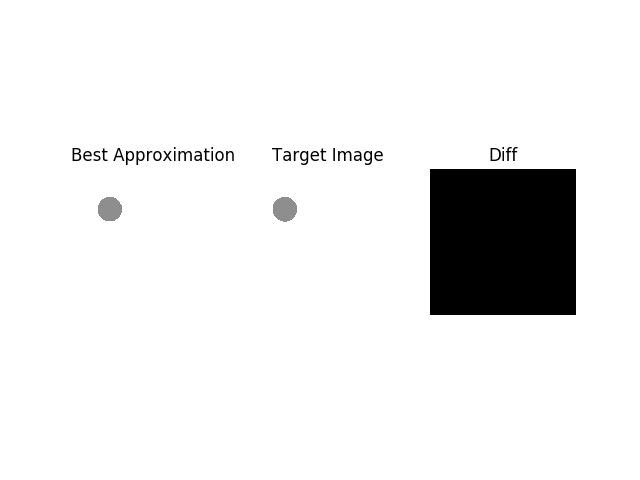
\includegraphics[width=0.7\textwidth]{output/evolve_perfect.png}
    \caption{Evolving a perfect approximation}\label{fig:perfect}
\end{figure}

We also struggled with the evolutionary algorithm minimizing the radius of each circle, effectively
evolving the background image. We also saw the algorithm evolving the background color by
minimizing all but one circle, and increasing that circle's radius until it covered the entire
image as shown in \autoref{fig:nothing}.

\begin{figure}[H]
    \centering
    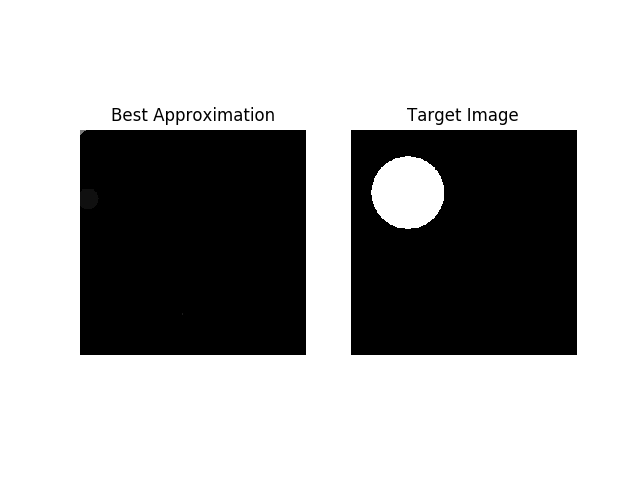
\includegraphics[width=0.7\textwidth]{output/evolve_nothing.png}
    \caption{Evolving the background color}\label{fig:nothing}
\end{figure}

Moving on to more complicated images, we saw that the algorithm would evolve the circles that
contribute the most to the image, but would minimize the rest. \autoref{fig:partial} shows some
examples of this.\footnote{Between runs we changed how the difference is computed and displayed.
    This is why one of them has a gray background and the other has a black background. Matplotlib
    by default uses a linear map between the least element and the greatest element of an array to
    determine what values correspond to what colors. If you take the difference between two images,
    you're likely to find fairly negative values and fairly positive values.} Note the tiny circles
present in the white background.

\begin{figure}[H]
    \centering
    \begin{subfigure}[b]{\textwidth}
        \centering
        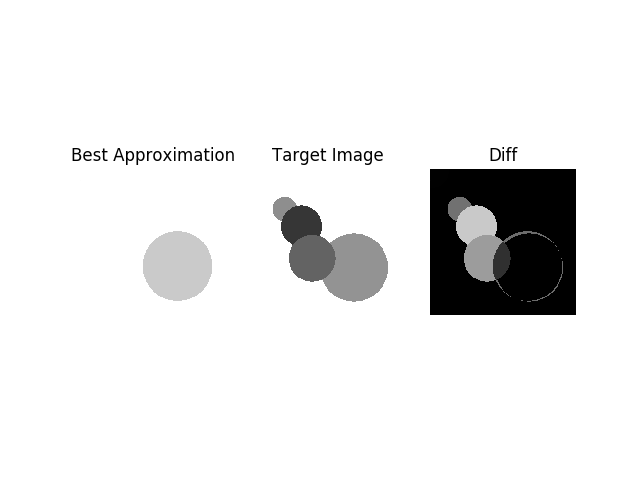
\includegraphics[width=0.6\textwidth]{output/evolve_one.png}
    \end{subfigure}
    \begin{subfigure}[b]{\textwidth}
        \centering
        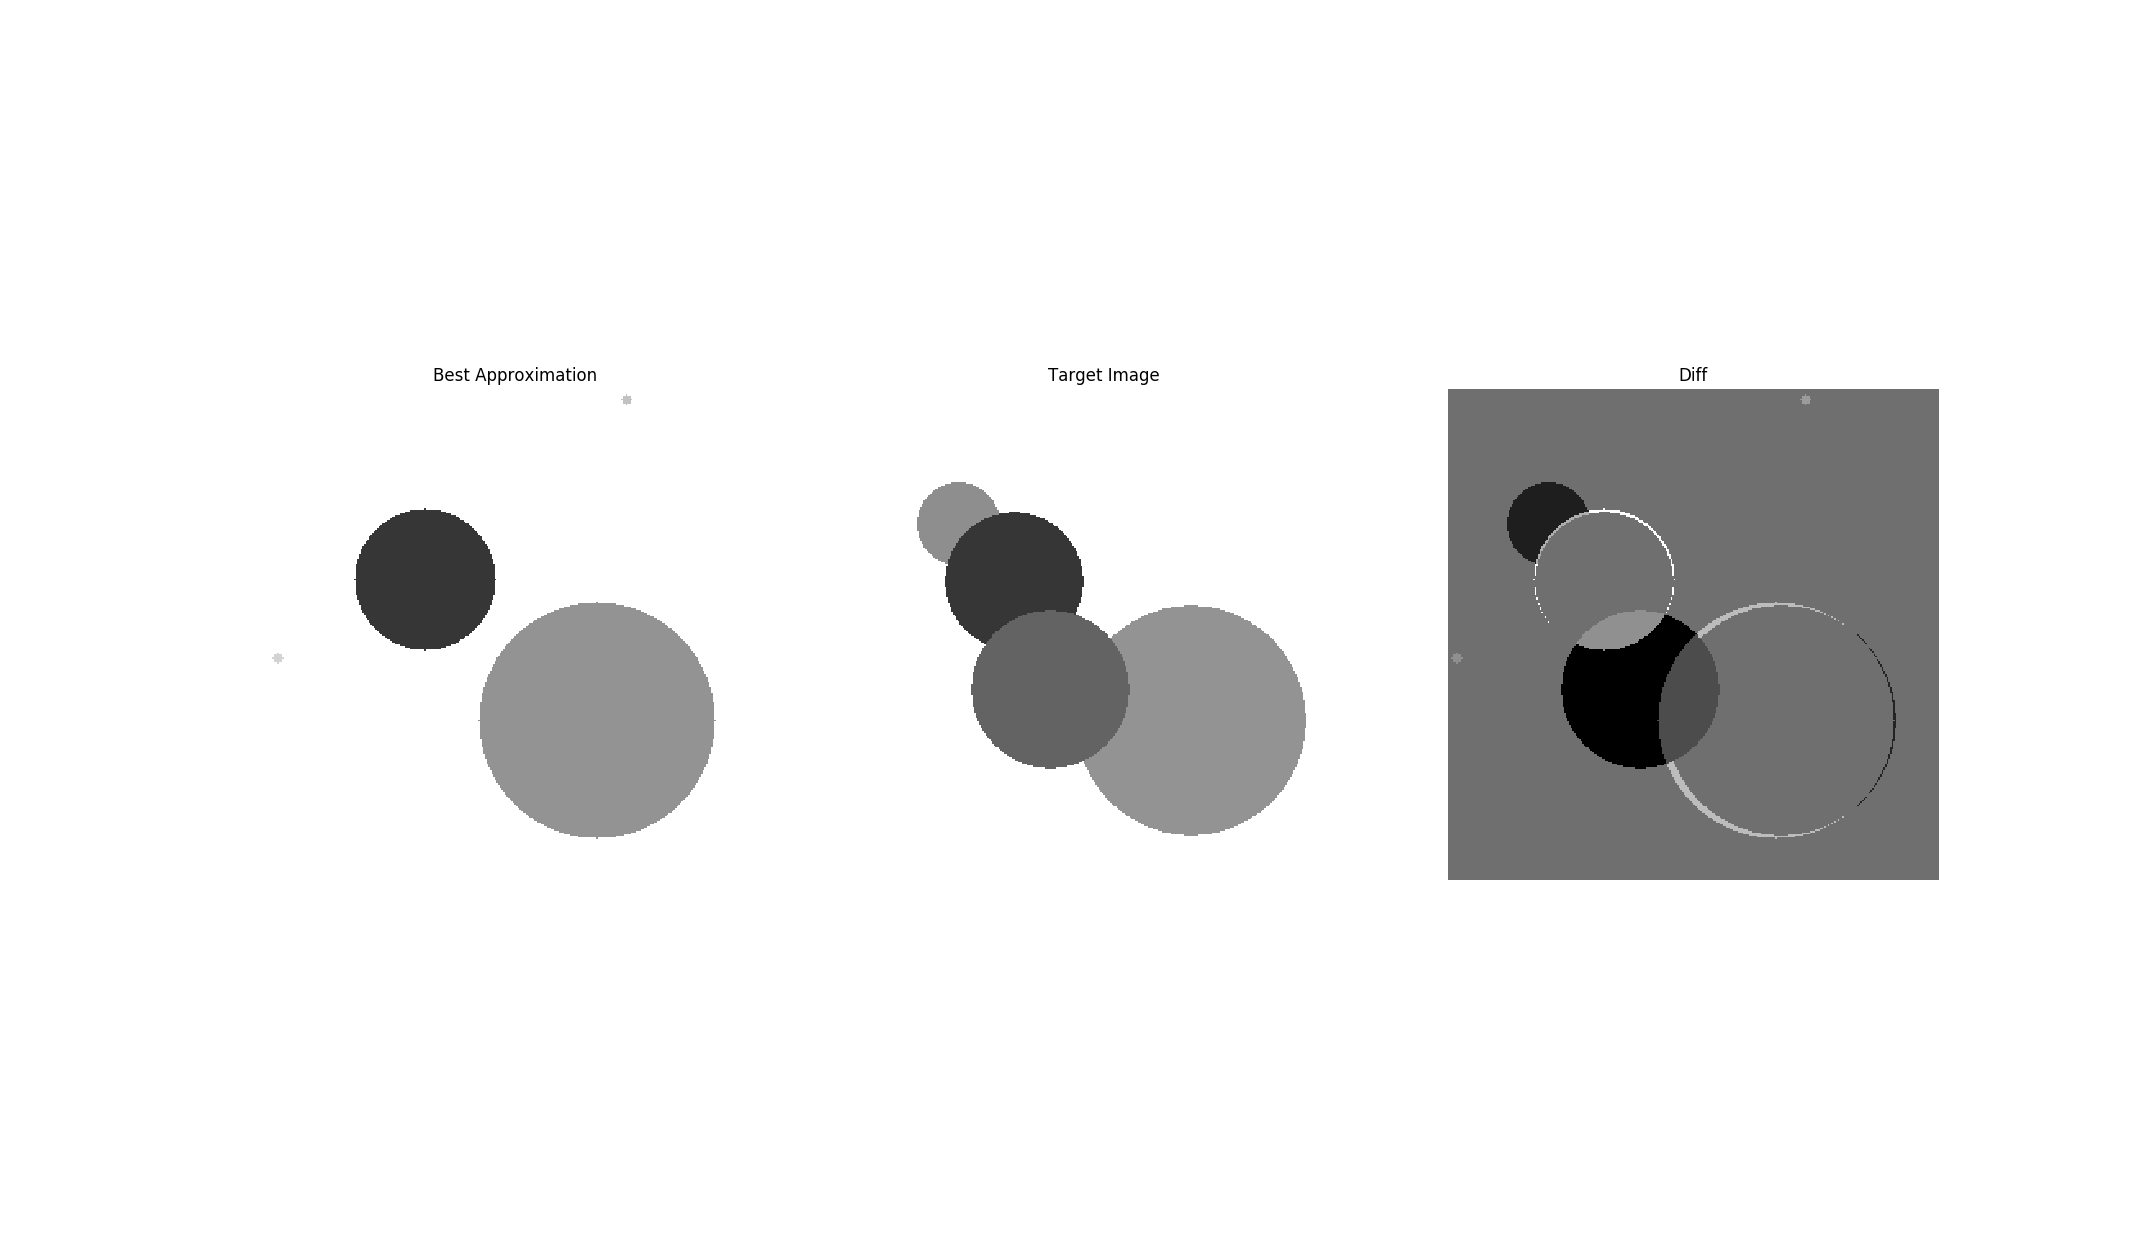
\includegraphics[width=0.6\textwidth]{output/evolve_some.png}
    \end{subfigure}
    \caption{Partial evolution of the images}\label{fig:partial}
\end{figure}

As mentioned in \autoref{sec:strat:evolutionary-algorithm}, we struggled with the circle center
mutation at times. We were never able to figure out why it was occurring, which was especially
difficult because \textit{exactly} the same code worked just fine in the
\autoref{alg:bootstrap-algorithm} implementation.

\begin{figure}[H]
    \centering
    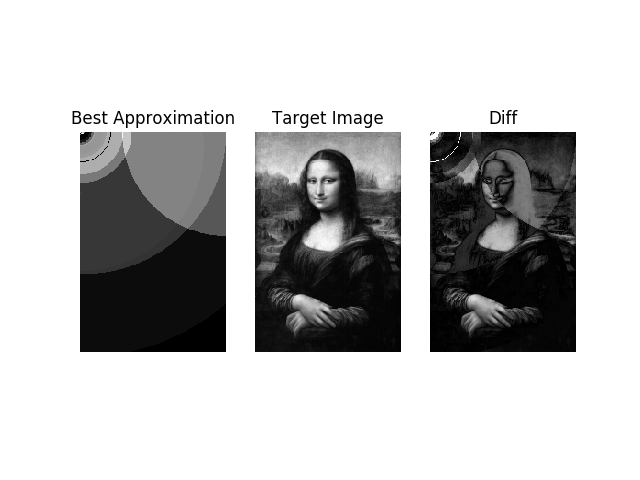
\includegraphics[width=0.7\textwidth]{output/ea-p100c200g400.png}
    \caption{The odd circle center mutations}\label{fig:center-mutations}
\end{figure}

Also note that the fitness of the best individual quickly converged over only a few generations as
indicated by \autoref{fig:ea-fitness-over-time}

\begin{figure}[H]
    \centering
    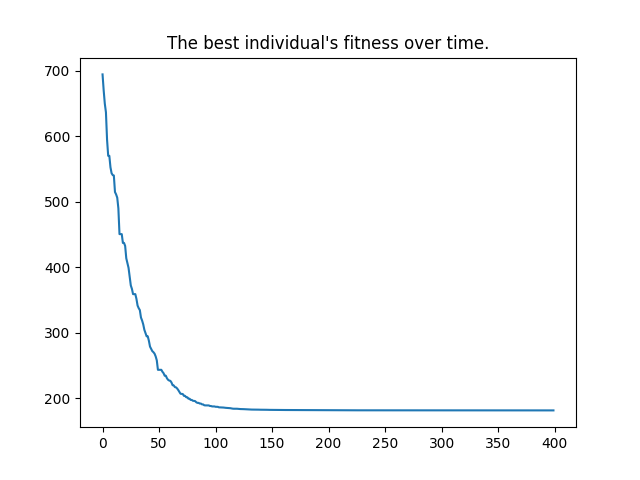
\includegraphics[width=0.7\textwidth]{output/ea-cooler-p100c200g400-fitness.png}
    \caption{Rapid convergence of the best fitness}\label{fig:ea-fitness-over-time}
\end{figure}

\subsection{A Combined Approach}\label{sec:results:combined-approach}
In view of the above results, and the desire to do something novel, we abandoned the standard
evolutionary algorithm in favor of kicking off an algorithm with an already good initial
population.

\begin{figure}[H]
    \centering
    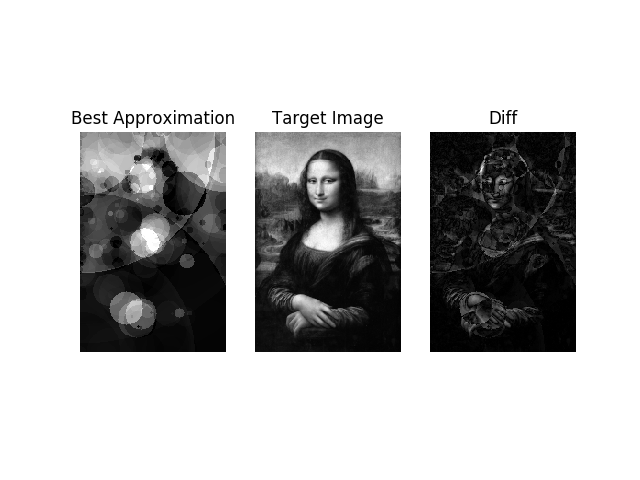
\includegraphics[width=0.7\textwidth]{output/ca-p256c400g2000.png}
    \caption{Results with a population of 256, 400 circles, and 2000
        generations}\label{fig:ca-p256-c400-g2000}
\end{figure}

\autoref{fig:ca-p256-c400-g2000} shows the results of a 10 hour overnight run of the combined
algorithm with a population of 256 individuals, 400 circles, and 2000 generations. We ran this
experiment without first attempting a smaller run to get a feel for how it behaved. The next
morning, we remembered that it would be good diagnostic information to plot the best fitness over
time, so we ran the algorithm again with more manageable numbers.

\begin{figure}[H]
    \centering
    \begin{subfigure}[b]{0.45\textwidth}
        \centering
        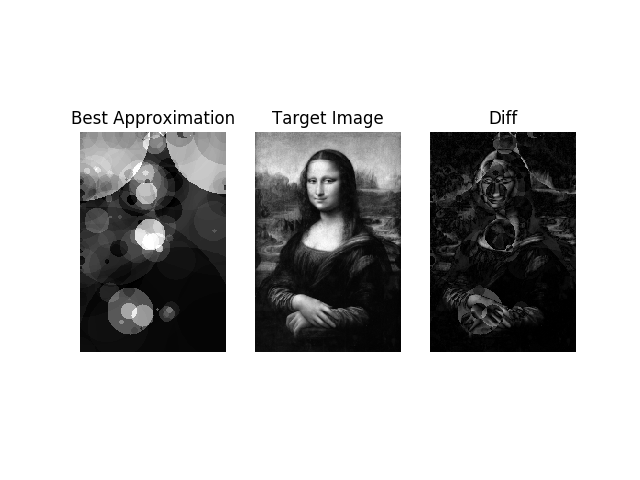
\includegraphics[width=\textwidth]{output/ca-p64c200g100.png}
    \end{subfigure}
    \begin{subfigure}[b]{0.45\textwidth}
        \centering
        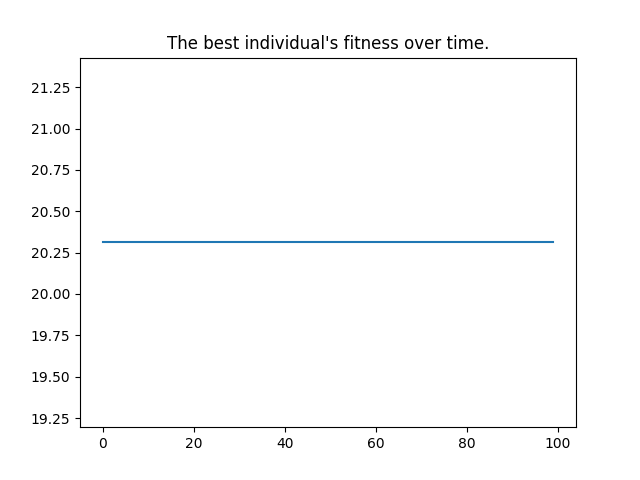
\includegraphics[width=\textwidth]{output/ca-p64c200g100-fitness.png}
    \end{subfigure}
    \caption{Results with a population of 64, 200 circles, and 100
        generations}\label{fig:ca-p64-c200-g100}
\end{figure}

As \autoref{fig:ca-p64-c200-g100} indicates, the algorithm did not improve the initial seed at all.
In fact, when the worst fitnesses were observed, they got steadily worse, by two orders of
magnitude. As discussed in \autoref{sec:strat:combined-approach}, we believe this is due to the
initial population not having enough diversity, resulting in us getting stuck in a local extremum.
Diversity is essential to the success of an evolutionary algorithm.

We identified multiple approaches to increasing the initial population diversity, but decided
against implementing them in favor of experimenting with the impact of the population size and
number of generations in running the circle-by-circle method.

\subsection{Circle by Circle}\label{sec:results:circle-by-circle}

Since printing the best and worst fitnesses at the end of each generation revealed that there was
so little diversity in the population, we decided to see what was the smallest population we could
use.

\begin{figure}[H]
    \centering
    \begin{subfigure}[b]{0.45\textwidth}
        \centering
        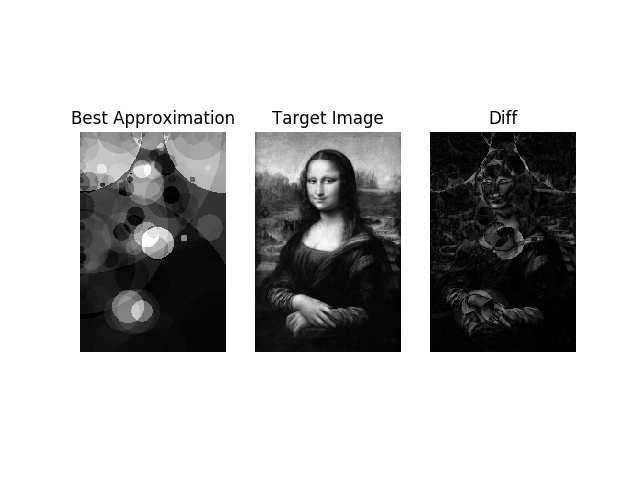
\includegraphics[width=\textwidth]{output/bs-p1c200g300.png}
        \caption{Results with population of 1, 200 circles, and 300 generations}
    \end{subfigure}
    \begin{subfigure}[b]{0.45\textwidth}
        \centering
        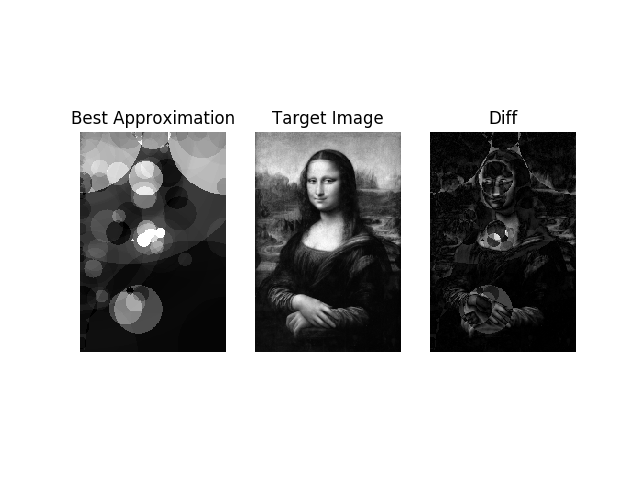
\includegraphics[width=\textwidth]{output/bs-p1c200g400.png}
        \caption{Results with population of 1, 200 circles, and 400 generations}
    \end{subfigure}
\end{figure}

\begin{figure}[H]
    \centering
    \begin{subfigure}[b]{0.45\textwidth}
        \centering
        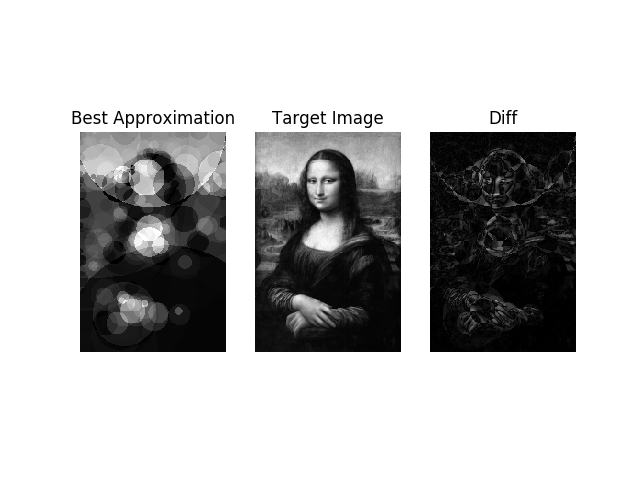
\includegraphics[width=\textwidth]{output/bs-p5c200g200.png}
        \caption{Results with population of 5, 200 circles, and 200 generations}
    \end{subfigure}
    \begin{subfigure}[b]{0.45\textwidth}
        \centering
        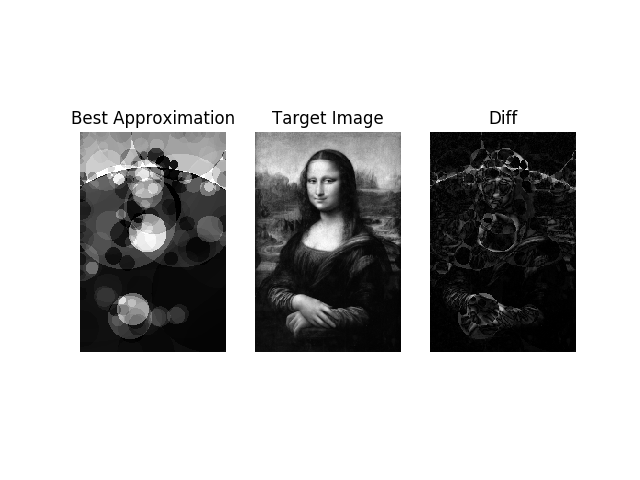
\includegraphics[width=\textwidth]{output/bs-p5c200g400.png}
        \caption{Results with population of 5, 200 circles, and 400 generations}
    \end{subfigure}
\end{figure}

This reveals that using small populations is a tenable approach to decreasing computation time,
while maintaining results.

Next, we held the population at a fixed large size, and attempted small numbers of generations.

\begin{figure}[H]
    \centering
    \begin{subfigure}[b]{0.45\textwidth}
        \centering
        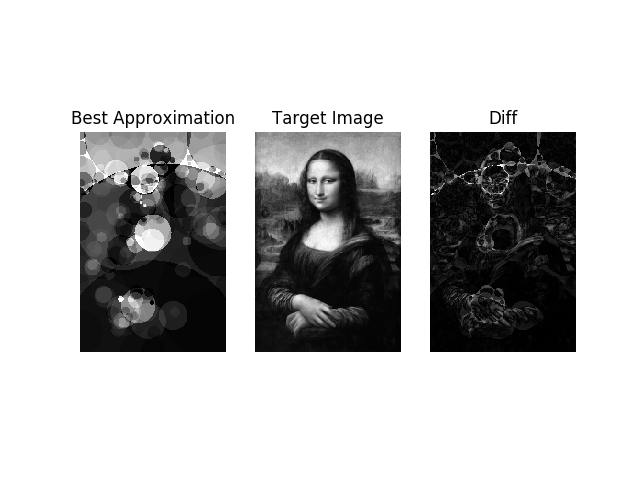
\includegraphics[width=\textwidth]{output/bs-p500c200g10.png}
        \caption{Results with population of 500, 200 circles, and 10 generations}
    \end{subfigure}
    \begin{subfigure}[b]{0.45\textwidth}
        \centering
        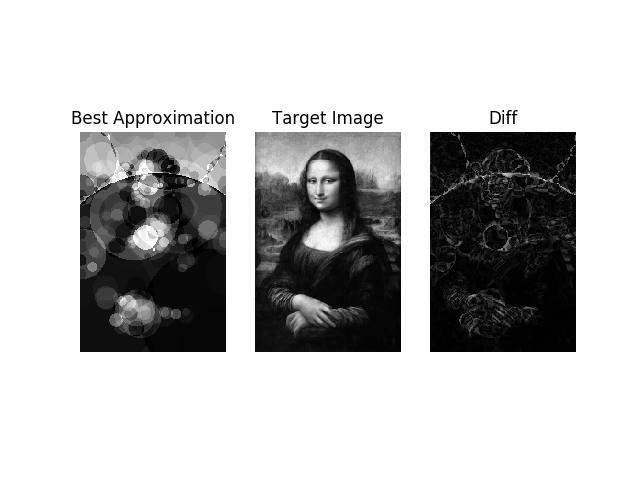
\includegraphics[width=\textwidth]{output/bs-p500c200g50.png}
        \caption{Results with population of 500, 200 circles, and 50 generations}
    \end{subfigure}
\end{figure}

This indicates that small numbers of generations yield okay results, but that it's better to have
more. The results with higher number of generations is looks less like abstract art and more like a
blurred version of the desired image. The highly scientific experiment of removing the author's
eyeglasses reveals that the image with 50 generations resembles the target the closest (At 12
inches from the screen, the image with 50 generations is indistinguishable from the target, while
the other is.)

Increasing the circle count, with a small population and small generation counts was the next task.

\begin{figure}[H]
    \centering
    \begin{subfigure}[b]{0.45\textwidth}
        \centering
        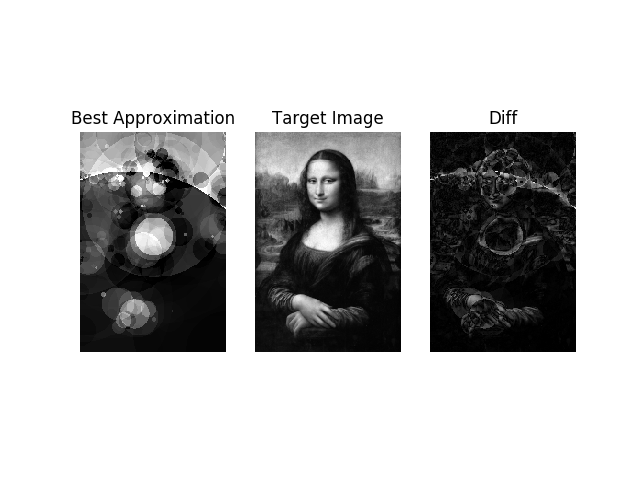
\includegraphics[width=\textwidth]{output/bs-p20c400g10.png}
        \caption{Results with population of 20, 400 circles, and 10 generations}
    \end{subfigure}
    \begin{subfigure}[b]{0.45\textwidth}
        \centering
        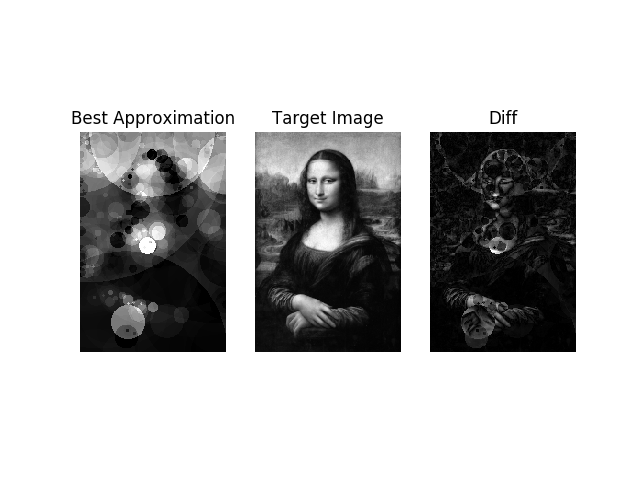
\includegraphics[width=\textwidth]{output/bs-p20c400g50.png}
        \caption{Results with population of 20, 400 circles, and 50 generations}
    \end{subfigure}
\end{figure}

This revealed that the bootstrap method is quite robust even with small populations and small
numbers of generations per circle. This means that it can be ran very quickly to get a good
approximation!

However note that the number of generations is more important than the population size. Higher
number of generations produce better approximations.

\begin{figure}[H]
    \centering
    \begin{subfigure}[b]{0.45\textwidth}
        \centering
        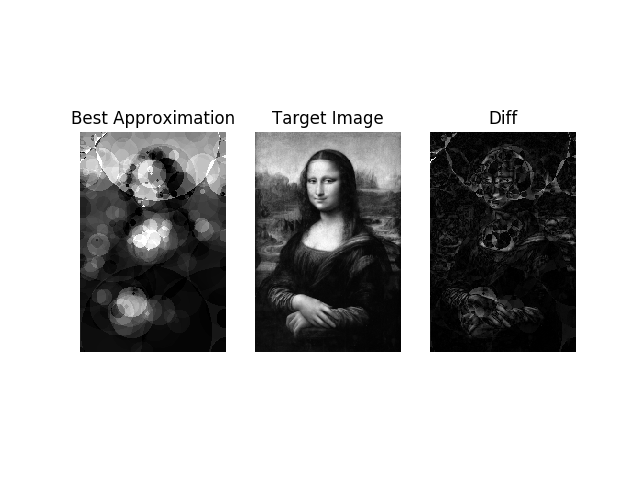
\includegraphics[width=\textwidth]{output/bs-p50c400g10.png}
        \caption{Results with population of 50, 400 circles, and 10 generations}
    \end{subfigure}
    \begin{subfigure}[b]{0.45\textwidth}
        \centering
        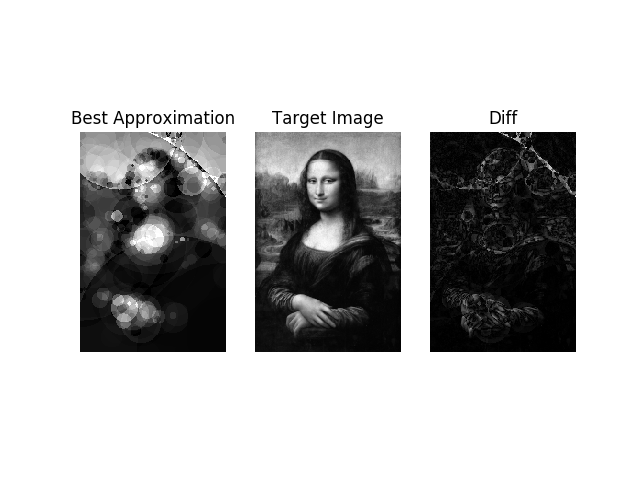
\includegraphics[width=\textwidth]{output/bs-p50c400g20.png}
        \caption{Results with population of 50, 400 circles, and 20 generations}
    \end{subfigure}
\end{figure}

\subsection{Individual Result Composition}

The last thing we played with was an idea we had at the beginning, but didn't have time. Since
parallelizing the bootstrap algorithm was so easy, we had the capability to run it multiple times
without the expensive cost of doing so. Since one approximation is good, many of them are better,
right? So we decided to composite several layers of results on top of each other to see if they
improved the results without greatly increasing computation time.

We expected small numbers of layers to give better approximations, and large numbers of layers to
effectively blur the image. In reality, the opposite happened.

\begin{figure}[H]
    \centering
    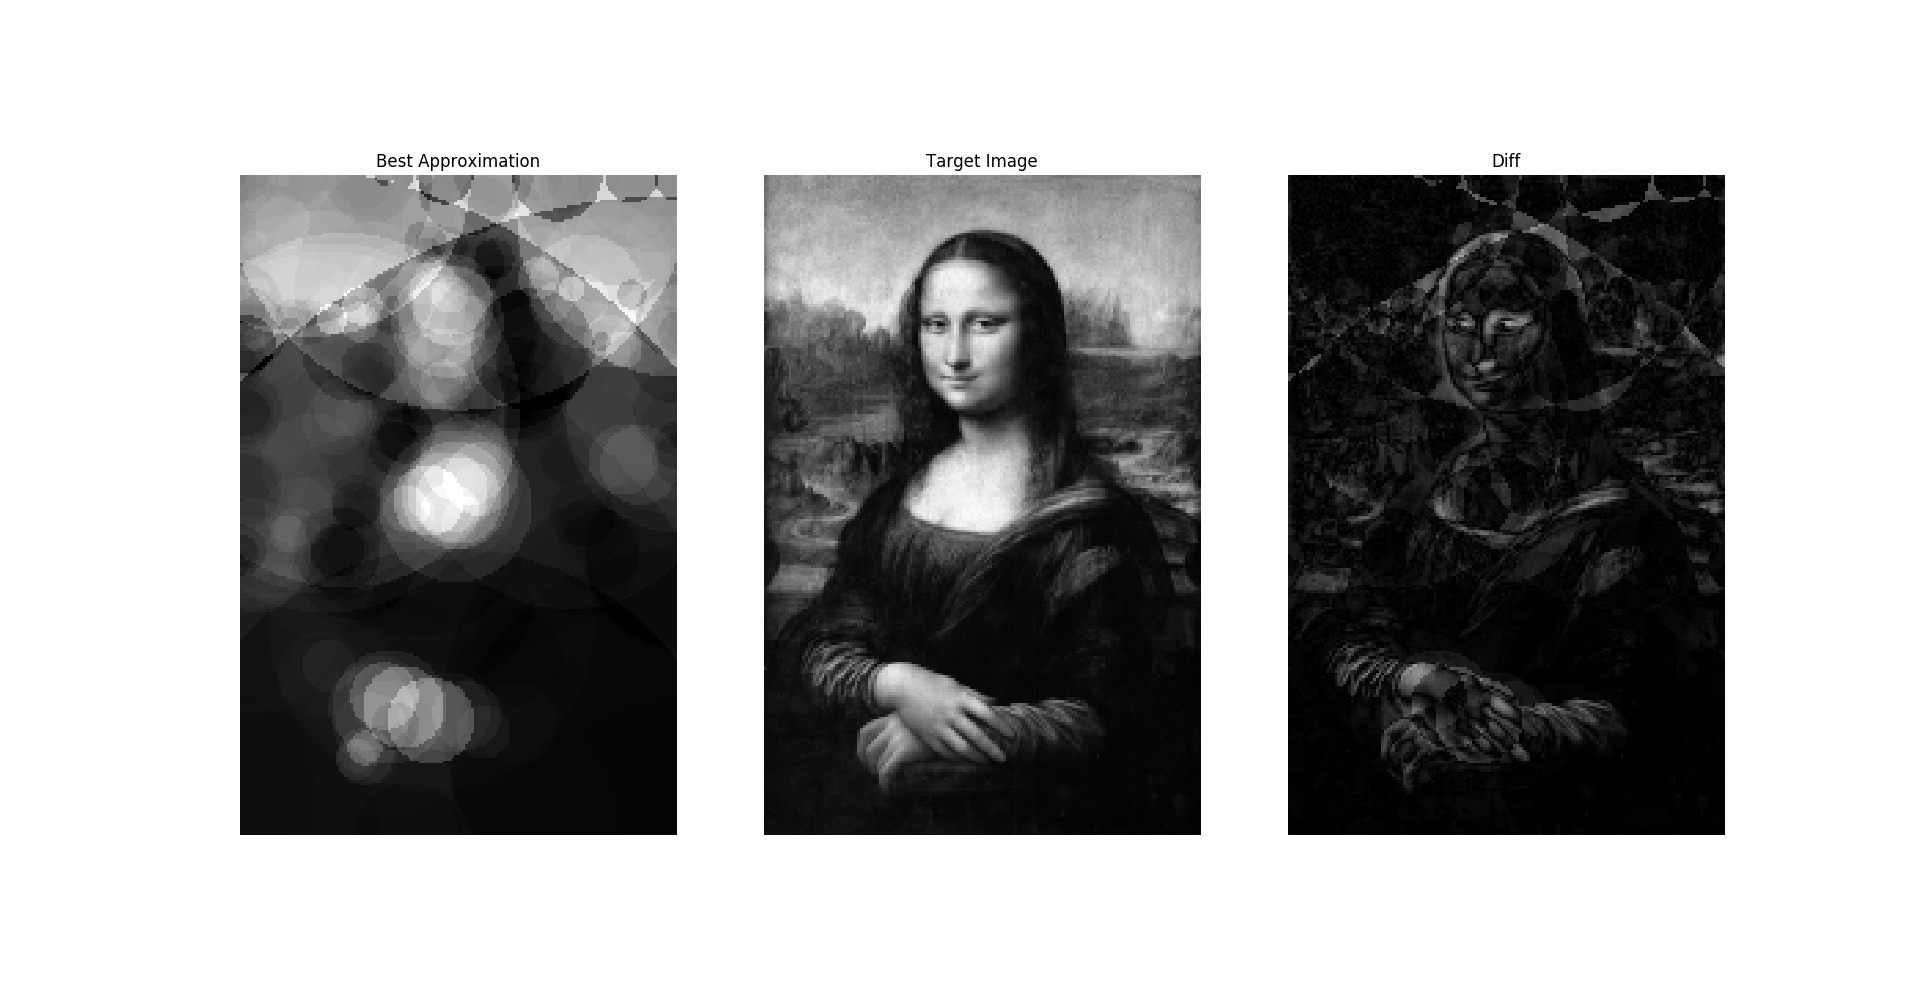
\includegraphics[width=\textwidth]{output/average3_c100p10g100.png}
    \caption{Three composite layers with population of 10, 100 circles, and 100
        generations}\label{fig:composite-3}
\end{figure}

\begin{figure}[H]
    \centering
    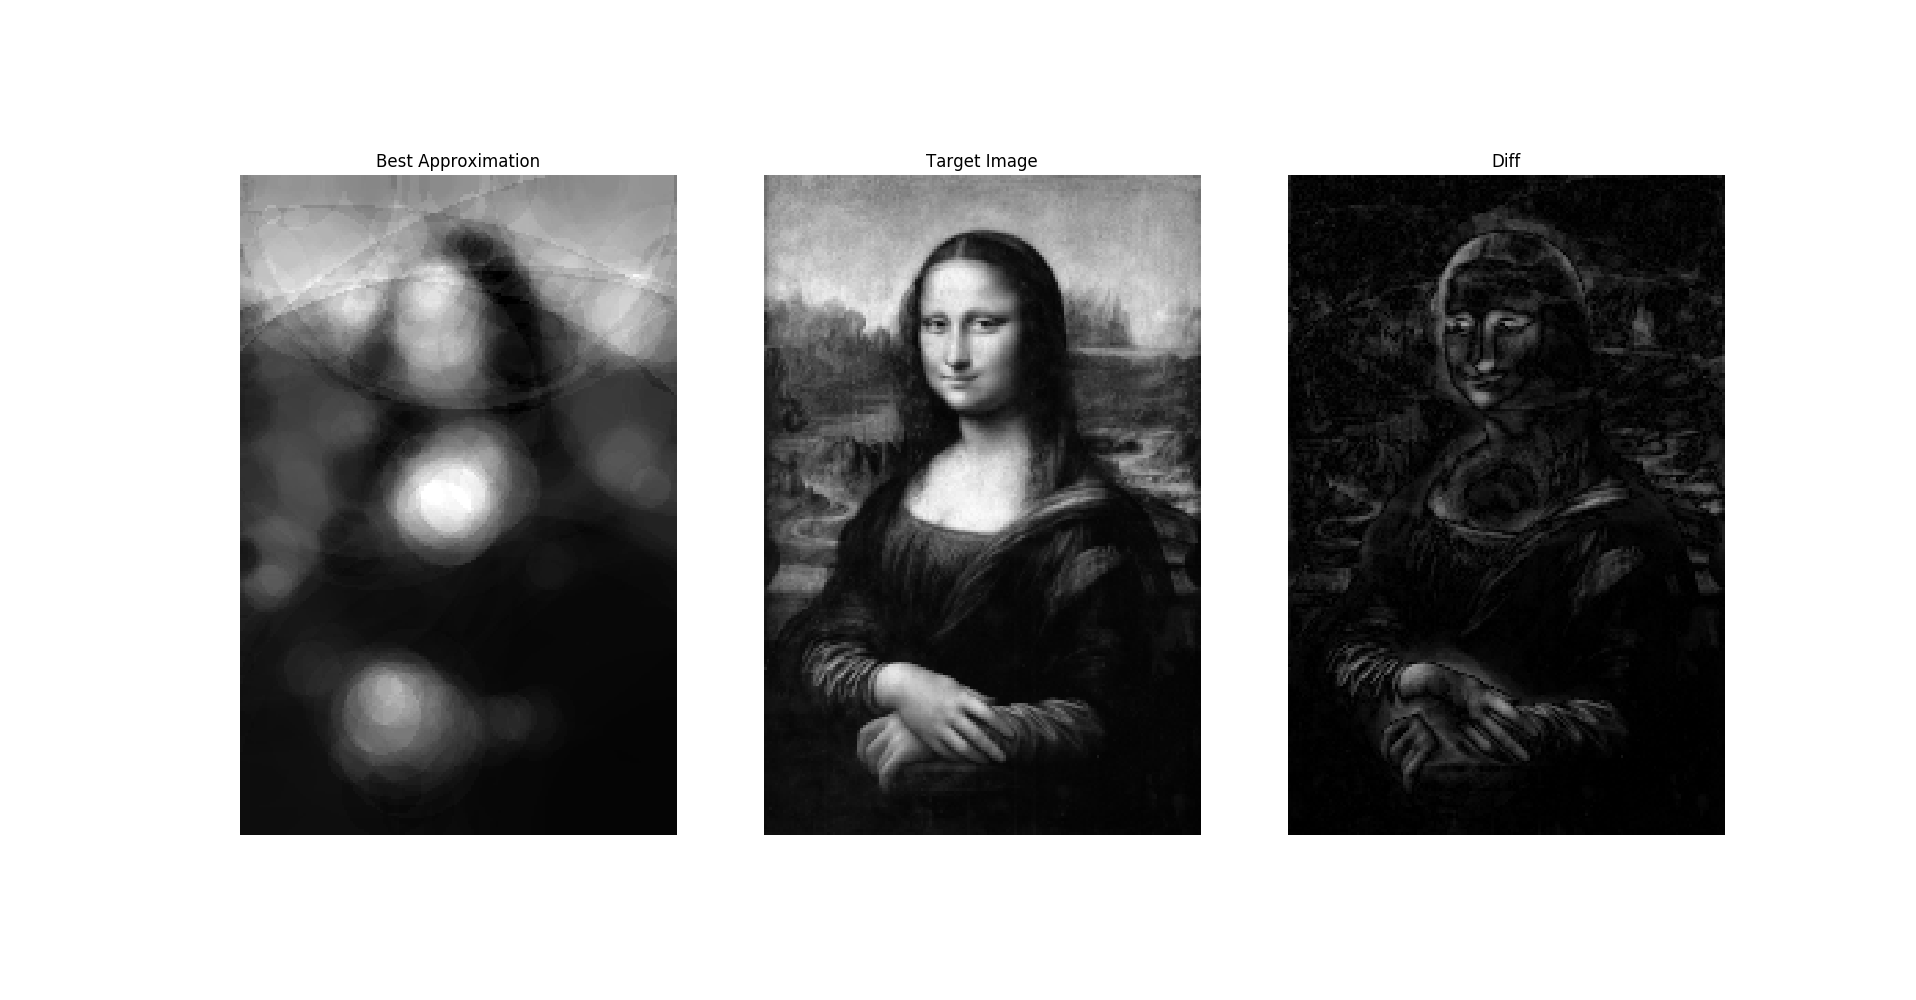
\includegraphics[width=\textwidth]{output/average_c100i10g100l64.png}
    \caption{64 composite layers with population of 10, 100 circles, and 100
        generations}\label{fig:composite-64}
\end{figure}

\begin{figure}[H]
    \centering
    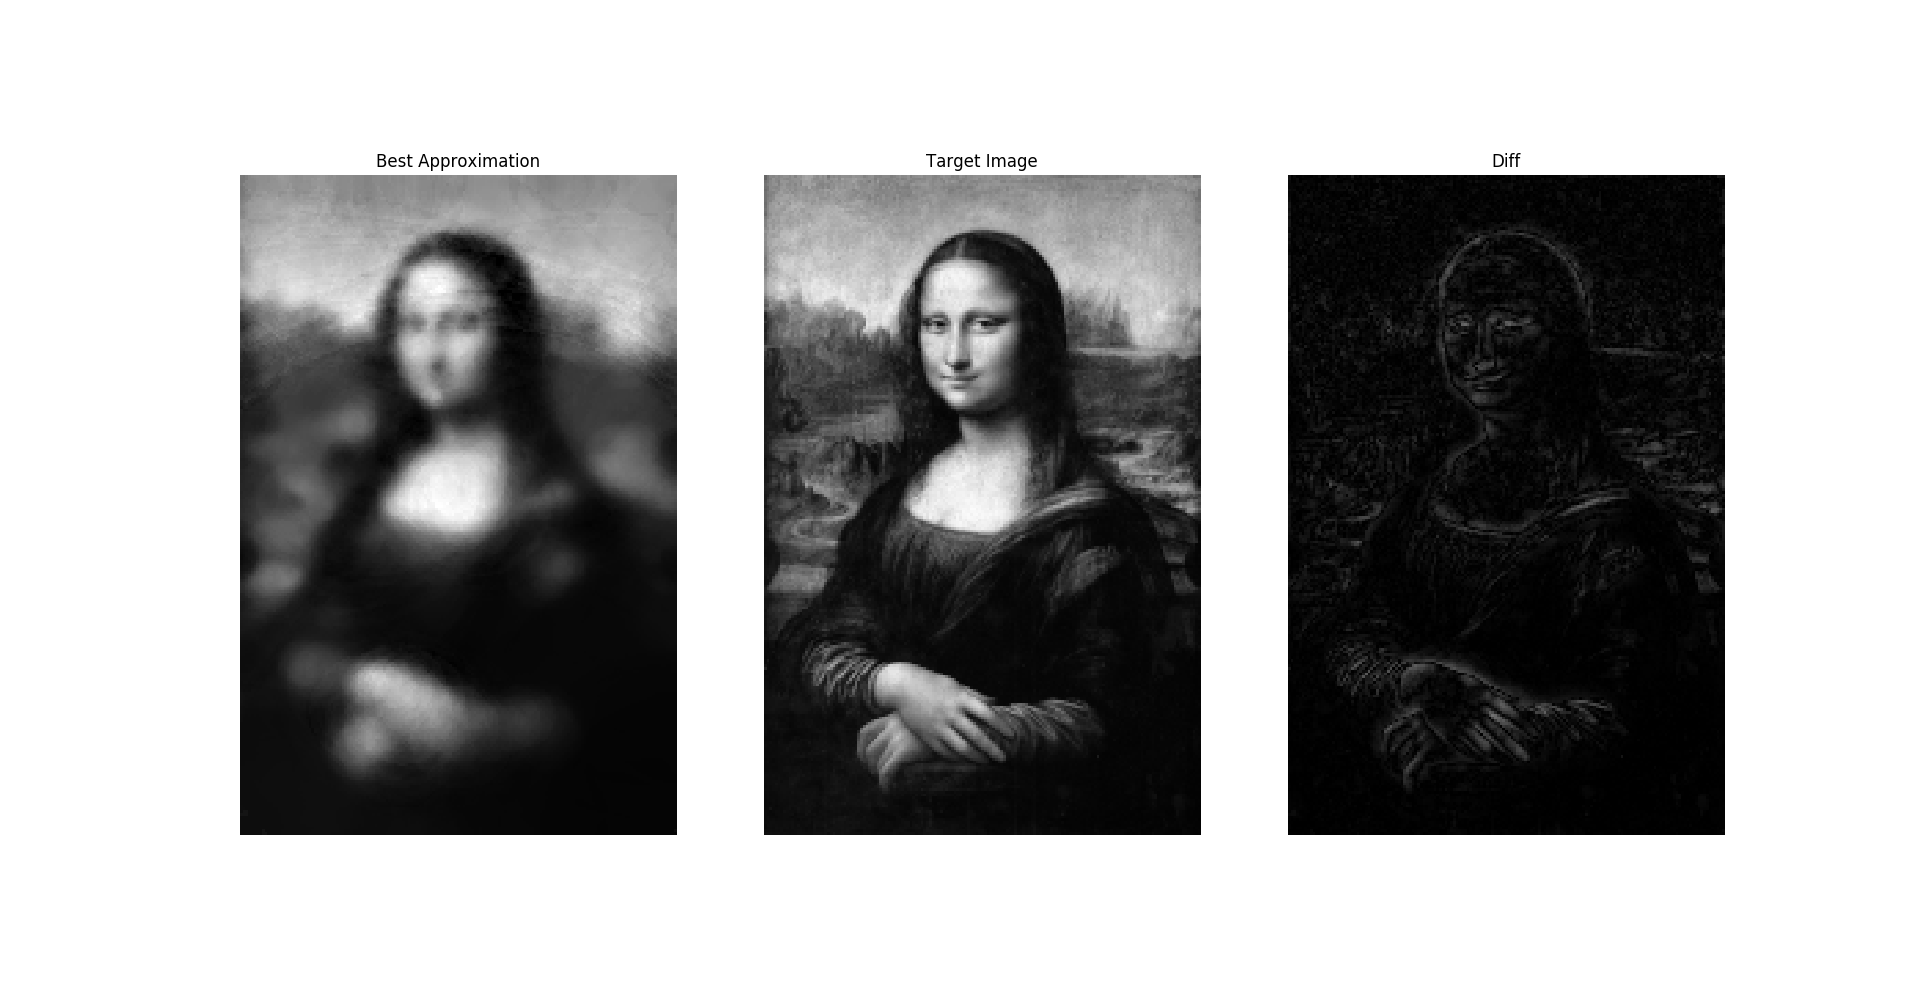
\includegraphics[width=\textwidth]{output/average32_c400p32g50.png}
    \caption{32 composite layers with population of 32, 400 circles, and 50
        generations}\label{fig:composite-32}
\end{figure}

\begin{figure}[H]
    \centering
    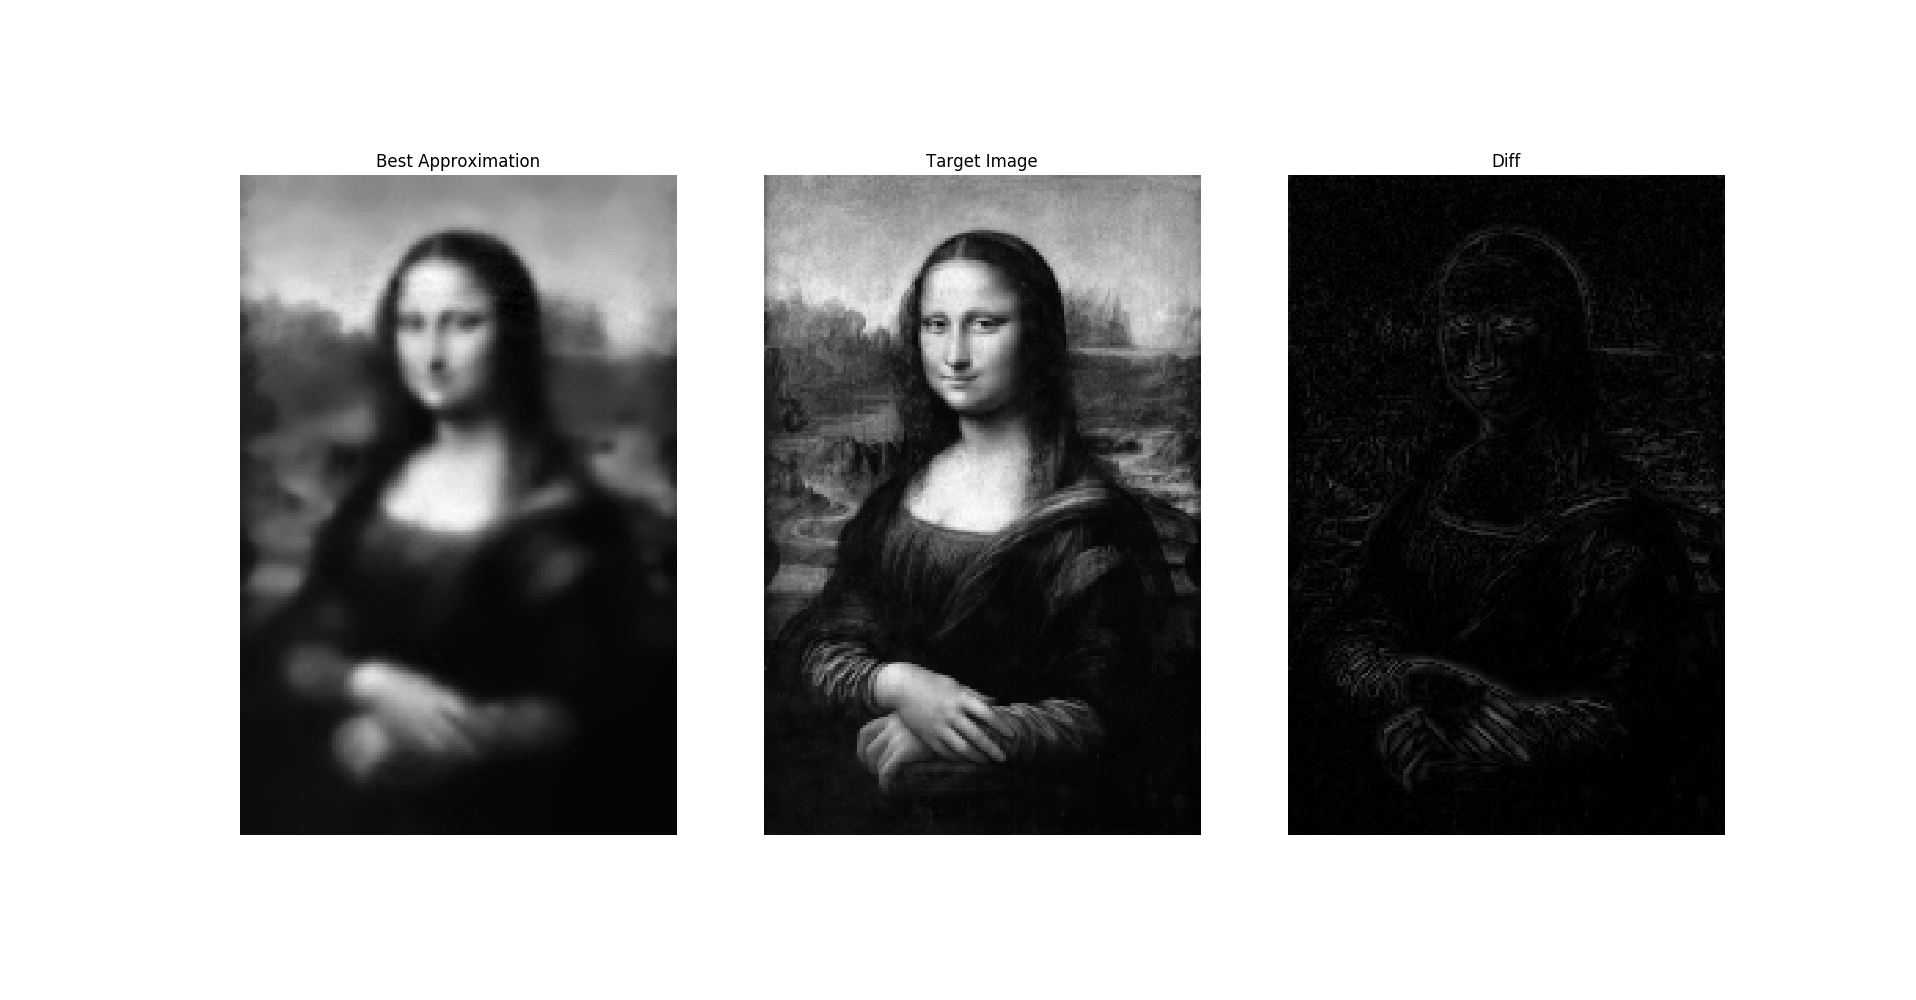
\includegraphics[width=\textwidth]{output/average64_c400p10g50l64.png}
    \caption{128 composite layers with population of 128, 400 circles, and 50
        generations}\label{fig:composite-128}
\end{figure}

The larger number of total circles in the end composite image produced the best approximation.

\section{Conclusion}
So to summarize our results, we struggled. The things we expected would work quite nicely failed to
yield reasonable results, and the things we expected to need more improvement worked quite well by
themselves.

There are many approaches we considered, and would like to have attempted, but could not due to
time constraints caused by work and other classes. We would have liked to have spent more time
tuning simulated annealing, because we still feel that it has the potential to yield excellent
results.

We also believe that it should be possible to use a simulated annealing-like approach to build an
approximation circle-by-circle. Our current method always takes the best individual circle at the
end of each generation. It may prove beneficial to take the best, or also accept a lesser fit
circle with some decreasing degree of randomness.

Our attempts at combining the two approaches --- building an approximation circle-by-circle and
evolving a population of such individuals --- did not prove useful, but we believe that increasing
the diversity of the initial population and improving the recombination operator and selection
method would have better results. We identified multiple ways to add diversity. First, we could use
a base individual (or individuals) and add \textit{more} circles to each, and evolve only those
additional circles. Second, we could increase the diversity by running the bootstrap initialization
for fewer generations, and with more randomness in the mutations. Third, we could only seed a few
members of the initial population, and leave the rest as randomly initialized.

Lastly, we had the idea of using a density based clustering algorithm like DBSCAN to identify
hotspots in the difference between the target image and the approximation. We could then use the
hotspots to identify which elements of the genome of a given individual contribute positively, and
which elements contribute negatively to the overall fitness of the individual. We are unsure at
this time if the additional computational requirements of repeated clustering would be worth it.
Especially as the clustering algorithms are typically fairly expensive.

Our final recommended approach to solving this problem is to use a computationally cheap method to
produce a largish number of individual approximations, and then to layer those approximations on
top of each other. Because there is no data dependency, the approximations can be produced in
parallel, and because there is diversity in the approximations, the composite result has greater
detail than each individual approximation.

\end{document}
